\newpage

\section{Detekcja źrenic}

W pracy dyplomowej występuje sterowanie aplikacją za pomocą ruch gałek ocznych, w szczególności analizując położenie źrenic. Mając wykryty obszar oczu (patrz rozdz. \hyperref[{section:eye_detection}]{\textit{\ref{section:eye_detection}.Detekcja oczu}}) metodami klasycznymi przetwarzania obrazów określam położenie środka źrenicy.
\par
W projekcie zaimplementowane zostały trzy algorytmy do testów i wybrany jeden, który dawał najlepsze rezultaty.

\subsection{Algorytm CDF (Cumulative Distribution Function)}
Algorytm zaimplementowany na podstawie dwóch artykułów o detekcji źrenic \cite{IMECSPupilCDFAnalysis}
\cite{EyePupilWebCam}. Opiera się w głównej mierze na progowaniu za pomocą dystrybuanty. Następnie analizuje najciemniejsze obszary, w których wyznacza środek źrenicy.

\iffalse
\begin{figure}[!h]
    \begin{center}
        \subfigure[Oko skierowane w prawo]{\label{fig:pupil_cdf_left}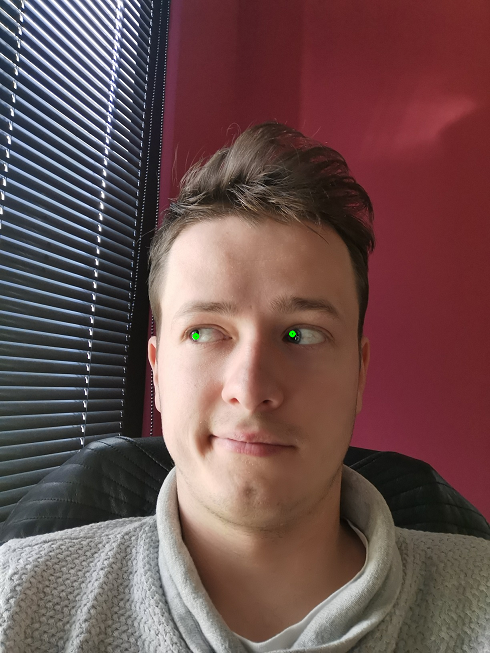
\includegraphics[scale=0.3]{img/pupil_section/pupil_2eyes_left_1.png}}
        \hspace{3mm}
        \subfigure[Oko skierowane na wprost]{\label{fig:pupil_cdf_center}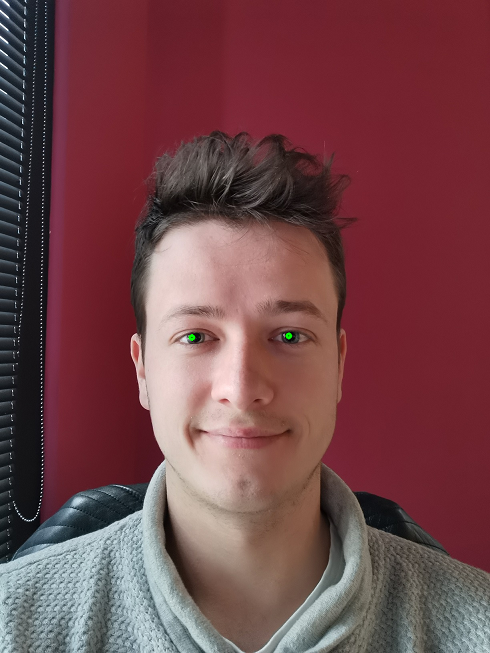
\includegraphics[scale=0.3]{img/pupil_section/pupil_2eyes_center_1.png}}
        \hspace{3mm}
        \subfigure[Oko skierowane w lewo]{\label{fig:pupil_cdf_right}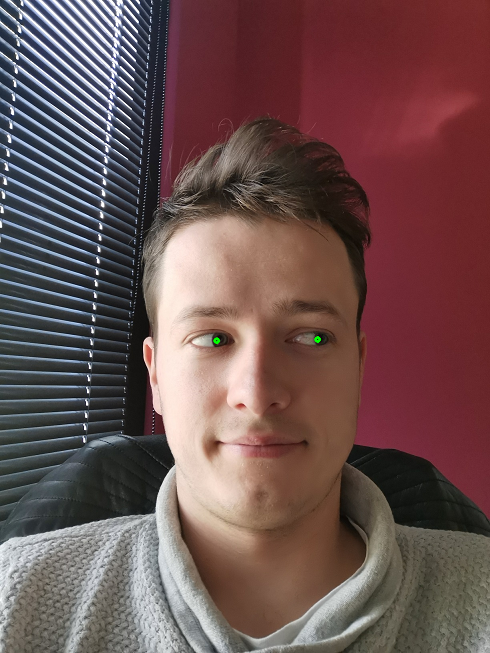
\includegraphics[scale=0.3]{img/pupil_section/pupil_2eyes_right_1.png}}
    \end{center}
    \caption{Rezultat wykrywania źrenic metodą CDF}
    \label{fig:cdf_results}
\end{figure}
\fi

\subsubsection{Kroki algorytmu}

\begin{itemize}
    \item Za pomocą progowania z użyciem dystrybuanty tworzymy obraz binarny.\\
    \begin{align}
        CDF(r) = \sum_{w=0}^{r} p(w)
    \end{align}
    
    Gdzie \textit{p(w)} to prawdopodobieństwo znalezienia punktu o jasności równej \textit{w} - określone przy pomocy dystrybuanty.
    
    \begin{align}
        I`(x, y) = 
        \begin{cases}
            255, &  CDF(I(x, y)) < \textit{a}\\
            0,   &  wpp
        \end{cases}
    \end{align} 
    
    Gdzie \textit{I} to jasność piksela, natomiast \textit{a} to ustalony próg

    \item Na uzyskany obraz binarny nakładamy operację morfologiczną erozji (filtr minimalny), celem usunięcia pojedynczych ciemnych pikseli
    
    \item Znajdujemy najciemniejszy piksel na oryginalnym obrazie wśród tych, które mają wartość 255 (są białe) na obrazie binarnym
    
    \item Obliczamy średnią jasność pikseli w kwadracie 10x10 wokół wybranego najciemniejszego punktu
    
    \item Nakładamy erozję na obszarze 15x15 wokół wybranego punktu
    \item Na tym obszarze stosujemy progowanie
    
    \begin{align}
        I`(x, y) = 
        \begin{cases}
            255, &  I(x, y) < I_{AVG}\\
            0,   &  wp.p.
        \end{cases}
    \end{align}
    
    Gdzie \textit{$I_{AVG}$} to średnia jasność obszaru obliczona wcześniej
    
    \item Środkiem źrenicy będzie środek ciężkości białych punktów na binarnym obszarze, który uzyskaliśmy

\end{itemize}

\iffalse
\begin{figure}[!h]
    \begin{center}
        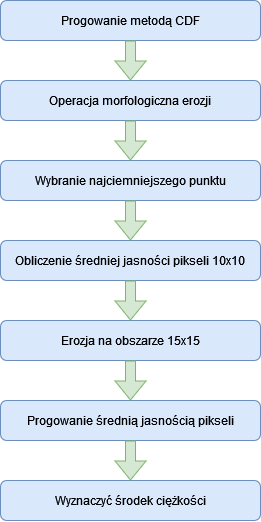
\includegraphics[scale=0.35]{img/pupil_section/CDF_Diagram.png}
        \caption{Kroki algorytmu metodą CDF}
        \label{fig:cdf_diagram}
    \end{center}
\end{figure}
\fi

\subsubsection{Wynik kolejnych etapów algorytmu}
Na \hyperref[{fig:cdf_steps}]{\textit{rys. \ref{fig:cdf_steps}}} przedstawiony jest wynik kolejnych etapów detekcji źrenic za pomocą metody \textit{CDF} na przykładowym zdjęciu oka.

\begin{figure}[!h]
    \begin{center}
        \subfigure[Obszar oka w skali szarości]{\label{fig:cdf_gray}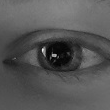
\includegraphics[scale=0.50]{img/pupil_section/CDF_steps/CDF_gray_eye.png}}
        \hspace{8mm}
        \subfigure[Wynik progowania CDF]{\label{fig:cdf_binary}
\includegraphics[scale=0.50]{img/pupil_section/CDF_steps/CDF_binary_eye_after_CDF.png}}
        \hspace{8mm}
        \subfigure[Wynik erozji]{\label{fig:cdf_erode}
\includegraphics[scale=0.50]{img/pupil_section/CDF_steps/CDF_binary_eye_after_erode.png}}
        
        \hfill
        
        \subfigure[Najciemniejszy punkt]{\label{fig:cdf_darkest}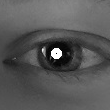
\includegraphics[scale=0.50]{img/pupil_section/CDF_steps/CDF_darkest_pixel.png}}
        \hspace{8mm}
        \subfigure[Obszar 10x10, w którym obliczana jest średnia jasność]{\label{fig:cdf_avgIntens}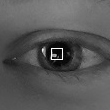
\includegraphics[scale=0.50]{img/pupil_section/CDF_steps/CDF_avgIntensity_region.png}}
        \hspace{8mm}
        \subfigure[Wynik erozji]{\label{fig:cdf_eroded}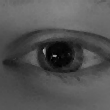
\includegraphics[scale=0.50]{img/pupil_section/CDF_steps/cdf_eroded_eye.png}}
        
        \hfill
        
        \subfigure[Obszar 15x15, który poddawany jest progowaniu]{\label{fig:cdf_pmi}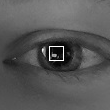
\includegraphics[scale=0.50]{img/pupil_section/CDF_steps/CDF_pmi.png}}
        \hspace{8mm}
        \subfigure[Progowanie średnią jasnością pikseli]{\label{fig:cdf_threshold}
\includegraphics[scale=3.65]{img/pupil_section/CDF_steps/CDF_threshold_pmi.png}}
        \hspace{8mm}
         \subfigure[Wykryte położenie źrenicy]{\label{fig:cdf_pupil_detected}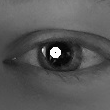
\includegraphics[scale=0.50]{img/pupil_section/CDF_steps/CDF_pupil_detected.png}}

        
    \end{center}
    \caption{Kolejne etapy wykrywania źrenic metodą CDF}
    \label{fig:cdf_steps}
\end{figure}

\subsection{Algorytm PF (Projection Function)}

Algorytm po raz pierwszy opisany w artykule zatytułowanym \textit{Projection Functions for Eye Detection} \cite{projection_function} z 2004 roku. Jest oparty na rzutowaniu jasności pikseli na składowe poziome i pionowe. Do obliczenia tych wartości wykorzystuje się funkcje projekcji, która może przyjmować różne postaci - z czego trzy zostały opisane w tej pracy dyplomowej. Największe różnice wartości oznaczają szybkie zmiany jasności, które mogą być konturami oka. \cite{EyePupilWebCam}

\subsubsection{Funkcja projekcji}

Funkcja projekcji służąca do rzutowania jasności rzędów i kolumn może przyjmować różne formy. Najczęściej stosowana jest funkcja całkowa, jednak ze względu na swoje niedociągnięcia i kłopoty z z wykrywaniem wariancji powstały także inne algorytmy. Trzy różne funkcje opisane są poniżej.

\paragraph{Funkcja całkowa} Wylicza się za jej pomocą średnią jasność pikseli w danym rzędzie lub kolumnie. W teorii jest to całka:
\begin{align}
    {IPF_h}(y) = \frac{1}{{x_b}-{x_a}}\int_{x_a}^{x_b} I(x,y) \, \mathrm{d}x
\end{align}
\begin{align}
    {IPF_v}(x) = \frac{1}{{y_b}-{y_a}}\int_{y_a}^{y_b} I(x,y) \, \mathrm{d}y
\end{align}

Ale w praktyce degeneruje się do funkcji sumy:

\begin{align}
    {IPF_h}(y)=\frac{1}{{x_b}-{x_a}}\sum_{x={x_a}}^{{x_b}} I(x,y)
\end{align}
\begin{align}
    {IPF_v}(x)=\frac{1}{{y_b}-{y_a}}\sum_{y={y_a}}^{{y_b}} I(x,y)
\end{align}

\paragraph{Funkcja wariancji} Średnia różnica między jasnością danego piksela, a wyliczonego \textit{IPF} danego rzędu lub kolumny

\begin{align}
    {VPF_h}(y)=\frac{1}{{x_b}-{x_a}}\sum_{x={x_a}}^{{x_b}} (I(x,y) - {IPF_h})
\end{align}
\begin{align}
    {VPF_v}(x)=\frac{1}{{y_b}-{y_a}}\sum_{y={y_a}}^{{y_b}} (I(x,y) - {IPF_v})
\end{align}

Chociaż we wskazanym wyżej artykule funkcja ta występuje w przedstawionej formie to spotykane są również postacie z różnicą kwadratową oraz z pierwiastkami z obliczonej wartości. 

\paragraph{Funkcja ogólna} Parametryzowana suma wyliczonych wartości \textit{IPF} i \textit{VPF}.

\begin{align}
    {GPF_h}(y)=(1-\alpha) * {IPF_h} + \alpha * {VPF_h}
\end{align}
\begin{align}
    {GPF_v}(x)=(1-\alpha) * {IPF_v} + \alpha * {VPF_v} 
\end{align}

Autorzy tej metody zalecają parametr $\alpha = 0.6$ jako dający najlepsze rezultaty.

\subsubsection{Kroki algorytmu}

\begin{itemize}
    \item Dla każdego rzędu i kolumny obliczamy wartość funkcji projekcji
    \item Dla wyliczonych funkcji projekcji obliczamy wartości pochodnej w każdym rzędzie i kolumnie
    \item Wybieramy po dwa ekstrema dla poziomego i pionowego wymiaru
    \item Przecięcie wybranych kolumn i rzędów utworzy prostokąt, którego środkiem będzie poszukiwany punkt na źrenicy 
\end{itemize}

\subsubsection{Wynik kolejnych etapów algorytmu}
Na \hyperref[{fig:pf_steps}]{\textit{rys. \ref{fig:pf_steps}}} przedstawiony jest wynik kolejnych etapów detekcji źrenic za pomocą metody \textit{PF} na przykładowym zdjęciu oka.

\begin{figure}[!h]
    \begin{center}
        \subfigure[Obszar oka w skali szarości]{\label{fig:pf_gray_eye}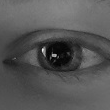
\includegraphics[scale=0.50]{img/pupil_section/PF_steps/PF_gray_eye.png}}
        \hspace{8mm}
        \subfigure[Pionowe wartości projekcji]{\label{fig:pf_x_projection}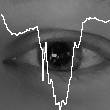
\includegraphics[scale=0.50]{img/pupil_section/PF_steps/PF_x_projection.png}}
        \hspace{8mm}
        \subfigure[Poziome wartości projekcji]{\label{fig:pf_y_projection}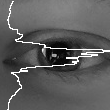
\includegraphics[scale=0.50]{img/pupil_section/PF_steps/PF_y_projection.png}}
        
        \hfill
        
        \subfigure[Pionowe wartości pochodnej]{\label{fig:pf_x_derviatives}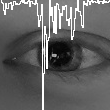
\includegraphics[scale=0.5]{img/pupil_section/PF_steps/PF_x_derivaties.png}}
        \hspace{8mm}
        \subfigure[Poziome wartości pochodnej]{\label{fig:pf_y_derviatives}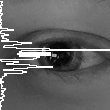
\includegraphics[scale=0.5]{img/pupil_section/PF_steps/PF_y_derivatives.png}}
        \hspace{8mm}
        \subfigure[Pionowe ekstrema]{\label{fig:pf_x_extremum}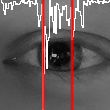
\includegraphics[scale=0.50]{img/pupil_section/PF_steps/PF_x_extremum.png}}
        
        \hfill
        
        \subfigure[Poziome ekstrema]{\label{fig:pf_y_extemum}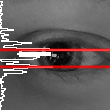
\includegraphics[scale=0.5]{img/pupil_section/PF_steps/PF_y_extremum.png}}
        \hspace{8mm}
        \subfigure[Środek wybranego obszaru]{\label{fig:pf_lines_intersection}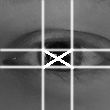
\includegraphics[scale=0.65]{img/pupil_section/PF_steps/PF_lines_intersection.png}}
        \hspace{8mm}
        \subfigure[Wykryte położenie źrenicy]{\label{fig:pf_pupil_detected}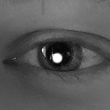
\includegraphics[scale=0.50]{img/pupil_section/PF_steps/PF_pupil_detected.png}}
        
    \end{center}
    \caption{Kolejne etapy wykrywania źrenic metodą PF}
    \label{fig:pf_steps}
\end{figure}

\subsection{Algorytm EA (Edge Analysis)}

Algorytm detekcji źrenic \cite{EyePupilWebCam} opierający się na wykryciu i analizie krawędzi. W teorii krawędzie najbardziej pionowe i poziome na zdjęciu powinny należeć do tęczówki i źrenicy.

\subsubsection{Kroki algorytmu}

\begin{itemize}
    \item Dla obszaru oka w skali szarości nakładamy filtr rozmywający, np. Gaussa. Pozwoli to pozbyć się drobnych szumów i wygładzić obraz.
    \item Wykrywamy krawędzie i tworzymy obraz binarny. Można zastosować np. algorytm Canny, który jest jedną z najpopularniejszych metod detekcji krawędzi
    \item Wybieramy dwa rzędy i dwie kolumny z największą liczbą punktów o wartości 255 (białe piksele na obrazie binarnym)
    \item Przecięcie wybranych rzędów i kolumn utworzy prostokąt, którego środkiem będzie poszukiwany punkt na źrenicy
\end{itemize}

\subsubsection{Wynik kolejnych etapów algorytmu}
Na \hyperref[{fig:ea_steps}]{\textit{rys. \ref{fig:ea_steps}}} przedstawiony jest wynik kolejnych etapów detekcji źrenic za pomocą metody \textit{EA} na przykładowym zdjęciu oka.

\begin{figure}[!h]
    \begin{center}
        \subfigure[Obszar oka w skali szarości]{\label{fig:ea_gray_eye}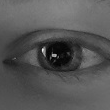
\includegraphics[scale=0.50]{img/pupil_section/EA_steps/EA_gray_eye.png}}
        \hspace{8mm}
        \subfigure[Rozmycie filtrem Gaussa]{\label{fig:ea_gaussian}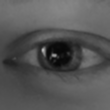
\includegraphics[scale=0.50]{img/pupil_section/EA_steps/EA_gaussian.png}}
        \hspace{8mm}
        \subfigure[Detekcja krawędzi metodą Canny]{\label{fig:ea_canny}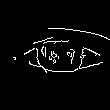
\includegraphics[scale=0.50]{img/pupil_section/EA_steps/EA_canny.png}}
        
        \hfill
        
        \subfigure[Najliczniejsze rzędy i~kolumny]{\label{fig:ea_canny_lines}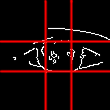
\includegraphics[scale=0.65]{img/pupil_section/EA_steps/EA_canny_lines.png}}
        \hspace{8mm}
        \subfigure[Środek wybranego obszaru]{\label{fig:ea_lines_intersection}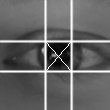
\includegraphics[scale=0.5]{img/pupil_section/EA_steps/EA_lines_intersection.png}}
        \hspace{8mm}
        \subfigure[Wykryte położenie źrenicy]{\label{fig:ea_pupil_detected}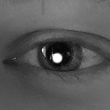
\includegraphics[scale=0.50]{img/pupil_section/EA_steps/EA_pupil_detected.png}}
    \end{center}
    \caption{Kolejne etapy wykrywania źrenic metodą EA}
    \label{fig:ea_steps}
\end{figure}